Thanks to the funds stored in the reserve pool, BitShares can offer to not only
pay for its own development and protocol improvement but also support and
encourage growth of an ecosystem.

In order to be get paid by BitShares, a proposal containing
\begin{inparaenum}[(a)]
 \item the date of work begin,
 \item the date of work end,
 \item a daily pay (denoted in BTS),
 \item the worker's name, and
 \item an internet address.
\end{inparaenum}
has to be publish on the blockchain and approved by shareholders.

A blockchain parameter (defined by shareholders through the committee) defines
the daily available budget. No more than that can be paid at any time to all so
called \emph{workers} combined.

The daily budget is distributed as illustrated in \cref{fig:workerpayalgo}: 
\begin{inparaenum}[(1)]
 \item The available budget is taken out of reserves pool.
 \item The budget items are sorted according to their approval rate
       ($v_\text{pro}-v_\text{con})$ in a descending order.
 \item Starting at the worker with the highest approval rate, the requested
       daily pay is payed until the daily budget is depleted.
 \item The worker with the least approval rate that was paid may receive less
       than the requested pay
\end{inparaenum}

\begin{figure}[!htp]
 \centering
  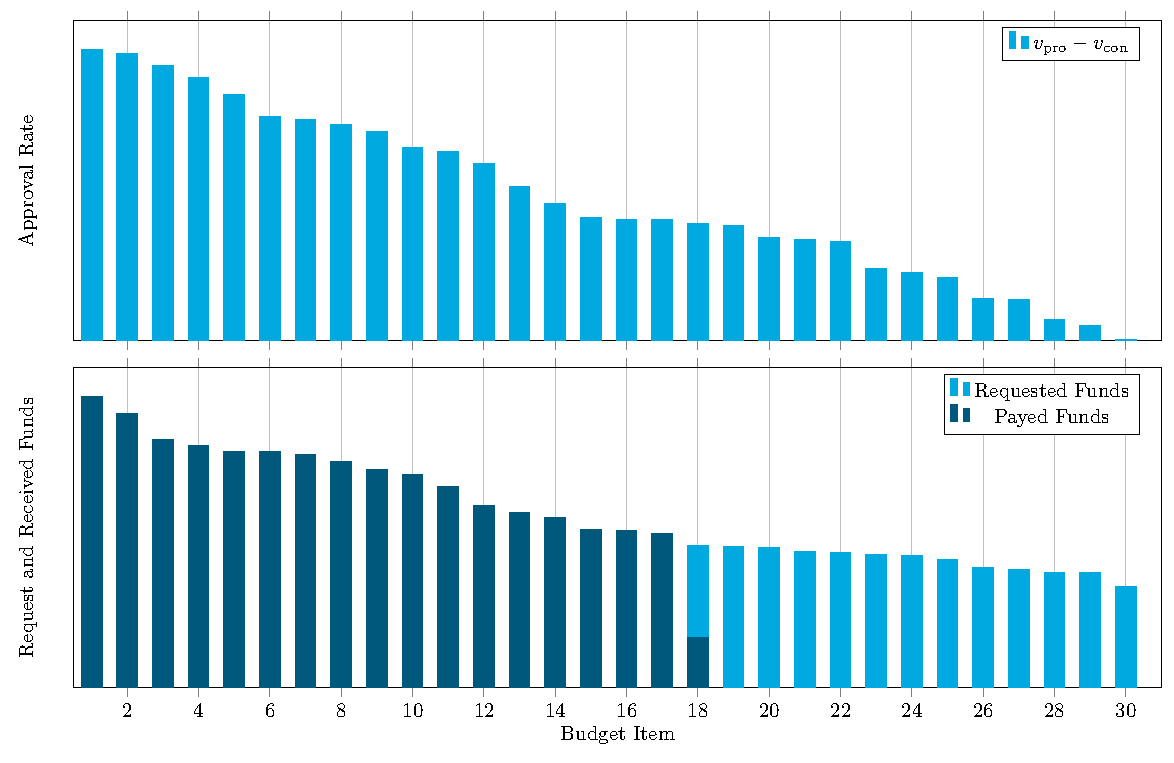
\includegraphics[width=\linewidth]{figures/worker-pay-algo.pdf}\vspace*{-2ex}
 \caption{Illustration of budget item payments.}
 \label{fig:workerpayalgo}
\end{figure}
Hence, in order to be successfully funded by the BitShares ecosystem, the
shareholder approval for your budget item needs to be highly ranked.

Since the payments for workers from the non-liquid reserve pool result in an
increased supply of BTS, these payments are vesting over a period of time
defined by shareholders.
